\documentclass[aspectratio=169,12pt]{beamer}
\usepackage[utf8]{inputenc}
\usepackage{amsmath, amssymb}
\usepackage{booktabs}
\usepackage{colortbl}
\usepackage{hyperref}
\usepackage{makecell}
\usepackage{ragged2e}
\usepackage{tikz}
\usetikzlibrary{arrows.meta, positioning, shapes.geometric, calc, tikzmark, shapes.misc, fit, decorations.pathreplacing}
\usepackage[siunitx, RPvoltages]{circuitikz}
\usepackage{tcolorbox}
\usepackage{array}
\usetheme{Madrid}

% Custom colors
\definecolor{correctgreen}{RGB}{0,150,0}
\definecolor{incorrectred}{RGB}{200,0,0}
\definecolor{counterblue}{RGB}{70,130,255}
\definecolor{highlightyellow}{RGB}{255,230,100}

% Address breakdown macro for showing tag/set/offset
\newcommand{\addressbreakdown}[3]{%
    \begin{tikzpicture}[
        section/.style={draw, very thick, minimum height=0.6cm},
        bitnumber/.style={font=\tiny},
        sectionlabel/.style={font=\scriptsize},
        baseline=(current bounding box.center)
    ]
    % Calculate total bits and positions
    \pgfmathtruncatemacro{\totalbits}{#1 + #2 + #3}
    \pgfmathtruncatemacro{\tagstart}{\totalbits - 1}
    \pgfmathtruncatemacro{\tagend}{\totalbits - #1}
    \pgfmathtruncatemacro{\setstart}{\tagend - 1}
    \pgfmathtruncatemacro{\setend}{\tagend - #2}
    \pgfmathtruncatemacro{\offsetstart}{\setend - 1}
    \pgfmathtruncatemacro{\offsetend}{0}

    % Scale factor for width
    \pgfmathsetmacro{\bitwidth}{0.17}

    % Starting position
    \pgfmathsetmacro{\xpos}{0}

    % Draw tag block
    \ifnum#1>0
        \pgfmathsetmacro{\tagwidth}{#1 * \bitwidth}
        \node[section, fill=blue!40, minimum width=\tagwidth cm] (tag) at (\xpos + \tagwidth/2, 0) {};
        \node[sectionlabel] at (tag.center) {tag};

        % Add bit numbers below
        \node[bitnumber] at ($(tag.south west) + (0mm,-1mm)$) {\tagstart};
        \node[bitnumber] at ($(tag.south east) + (-1mm,-1mm)$) {\tagend};

        \pgfmathsetmacro{\xpos}{\xpos + \tagwidth}
    \fi

    % Draw set block
    \ifnum#2>0
        \pgfmathsetmacro{\setwidth}{#2 * \bitwidth}
        \node[section, fill=green!40, minimum width=\setwidth cm] (set) at (\xpos + \setwidth/2, 0) {};
        \ifnum#2<3
            \node[sectionlabel, rotate=90] at (set.center) {set};
        \else
            \node[sectionlabel] at (set.center) {set};
        \fi

        % Add bit numbers below
        \node[bitnumber] at ($(set.south west) + (1mm,-1mm)$) {\setstart};
        \node[bitnumber] at ($(set.south east) + (-1mm,-1mm)$) {\setend};

        \pgfmathsetmacro{\xpos}{\xpos + \setwidth}
    \fi

    % Draw offset block
    \ifnum#3>0
        \pgfmathsetmacro{\offsetwidth}{#3 * \bitwidth}
        \node[section, fill=yellow!40, minimum width=\offsetwidth cm] (offset) at (\xpos + \offsetwidth/2, 0) {};
        \ifnum#3<3
            \node[sectionlabel, rotate=90, font=\tiny] at (offset.center) {offset};
        \else
            \node[sectionlabel] at (offset.center) {offset};
        \fi

        % Add bit numbers below
        \ifnum#2>0
            \node[bitnumber] at ($(offset.south west) + (1mm,-1mm)$) {\offsetstart};
        \else
            % When no set bits, offset starts directly after tag
            \pgfmathtruncatemacro{\offsetstartalt}{\tagend - 1}
            \node[bitnumber] at ($(offset.south west) + (1mm,-1mm)$) {\offsetstartalt};
        \fi
        \node[bitnumber] at ($(offset.south east) + (0mm,-1mm)$) {\offsetend};
    \fi
    \end{tikzpicture}
}

\title{Branch Prediction}
\author{Computer Architecture 2340267}
\date{2025, Recitation \#6}
\begin{document}

\frame{\titlepage}

%==========================================
% Slide: Branch Prediction Overview
\begin{frame}
  \frametitle{Branch Prediction (Reminder)}

  \begin{center}
    \scalebox{0.7}{
    \begin{tikzpicture}[
      stage/.style={draw=blue!40, line width=1pt, minimum height=1cm, minimum width=1.5cm, fill=blue!10, font=\large, text=blue!80, rounded corners=2pt},
      latch/.style={draw=black!70, thick, fill=yellow!30, minimum width=0.25cm, minimum height=4.5cm},
      component/.style={draw=black!80, line width=1pt, fill=cyan!20, font=\small},
      btb/.style={draw=black!80, line width=1.5pt, minimum height=1cm, minimum width=1.2cm, fill=green!40, font=\small\bfseries},
      arrow/.style={->, >=stealth, thick},
      data_connector/.style={circle, fill, inner sep=1.2pt}
    ]

      % Instruction Memory - starting point (1.5x bigger)
      \node[muxdemux, muxdemux def={Lh=3, Rh=3, w=3, NL=1, NR=1},
            external pins width=0, fill=cyan!20] (imem) {};
      \node[font=\small, align=center] at (imem.center) {Instruction\\Memory};

      % Latch L1 - to the right of Instruction Memory
      \node[latch, anchor=west] at ([xshift=5mm]imem.rpin 1) (L1) {};

      % Register File - to the right of L1 (1.5x bigger)
      \node[muxdemux, muxdemux def={Lh=3, Rh=3, w=3, NL=4, NR=2},
            external pins width=0, fill=cyan!20, anchor=lpin 2] at ([xshift=6mm]L1.east |- imem.rpin 1) (regfile) {};
      \node[font=\small, align=center] at (regfile.center) {Register\\File};

      % Latch L2 - to the right of Register File
      \node[latch, anchor=west] at ([xshift=5mm]regfile.rpin 1 |- L1) (L2) {};

      % ALU - to the right of L2 (1.5x bigger)
      \node[muxdemux, muxdemux def={Lh=7.5, NL=2, Rh=3, NR=1, NB=2, NT=1, w=3, inset w=1.5, inset Lh=3, inset Rh=0, square pins=1},
            external pins width=0, scale=0.4, fill=cyan!20, anchor=lpin 1] at ([xshift=10mm]L2.east |- regfile.rpin 1) (alu) {};
      \node[rotate=90, font=\small] at ([xshift=1mm]alu.center) {ALU};

      % Latch L3 - to the right of ALU
      \node[latch, anchor=west] at ([xshift=5mm]alu.east |- L1) (L3) {};

      % Data Memory - to the right of L3 (1.5x bigger)
      \node[muxdemux, muxdemux def={Lh=3, Rh=3, w=3, NL=3, NR=1},
            external pins width=0, fill=cyan!20, anchor=lpin 1] at ([xshift=5mm]L3.east |- alu.rpin 1) (dmem) {};
      \node[font=\small, align=center] at (dmem.center) {Data\\Memory};

      % Latch L4 - to the right of Data Memory
      \node[latch, anchor=west] at ([xshift=5mm]dmem.rpin 1 |- L1) (L4) {};

      % WB Mux - to the right of L4 (1.5x bigger)
      \node[muxdemux, muxdemux def={Lh=6, Rh=3, NL=2, NR=1, w=1.5},
            external pins width=0, scale=0.6, fill=cyan!20, anchor=lpin 1] at ([xshift=8mm]L4.east |- dmem.rpin 1) (wb_mux) {};

      % Pipeline stages at top - north aligned with latches

      \node[stage, anchor=north] (id_stage) at ($(L1.north)!0.5!(L2.north)$) {ID};
      \node[stage, anchor=north] (if_stage) at (id_stage.north -| imem) {IF};
      \node[stage, anchor=north] (ex_stage) at ($(L2.north)!0.5!(L3.north)$) {EX};
      \node[stage, anchor=north] (mem_stage) at ($(L3.north)!0.5!(L4.north)$) {MEM};
      \node[stage, anchor=north] (wb_stage) at (mem_stage.north -| wb_mux) {WB};

      % BTB - positioned below Instruction Memory
      \node[btb, below=0.8cm of imem] (btb) {BTB};
      \draw[red!70, line width=2.5pt] (btb) ellipse [x radius=1cm, y radius=0.7cm];

      % Main wiring
      % IF to L1
      \draw[arrow] (imem.east) -- (L1.west);

      % L1 to Register File
      \draw[arrow] (L1.east) -- ++(0.3,0) |- (regfile.lpin 1);
      \draw[arrow] (L1.east) -- (regfile.lpin 2);

      % Register File to L2
      \draw[arrow] (regfile.rpin 1) -- (L2.west |- alu.lpin 1);
      \draw[arrow] (regfile.rpin 2) -- (L2.west |- regfile.rpin 2);

      % L2 to ALU
      \draw[arrow] (L2.east |- regfile.rpin 1) -- (alu.lpin 1);
      \draw[arrow] (L2.east |- regfile.rpin 2) -- ++(0.3,0) |- (alu.lpin 2);

      % L2 to L3
      \node[data_connector] at ([xshift=3mm]L2.east |- alu.lpin 2) (alu_conn) {};
      \draw[arrow] (alu_conn) |- (L3.west |- dmem.lpin 3); 
      %\draw[arrow] (L2.east |- alu.lpin 1) -- (L3.west);

      % ALU to L3
      \draw[arrow] (alu.rpin 1) -- (L3.west |- alu.rpin 1);

      % L3 to Data Memory
      \draw[arrow] (L3.east |- alu.rpin 1) -- (dmem.lpin 1);
      \node[data_connector] at ([xshift=2mm]L3.east |- alu.rpin 1) (dmem_conn) {};
      \draw[arrow] (dmem_conn) |- (dmem.lpin 2);
      \draw[arrow] (L3.east |- dmem.lpin 3) -- (dmem.lpin 3);

      % Data Memory to L4
      \draw[arrow] (dmem.rpin 1) -- (L4.west |- wb_mux.lpin 1);
      \node[data_connector] at ([xshift=2mm]L3.east |- dmem.rpin 2) (dmem_conn2) {};
      \draw[arrow] (dmem_conn2) |- (L4.west |- wb_mux.lpin 2);

      % L4 to WB Mux
      \draw[arrow] (L4.east |- dmem.rpin 1) -- (wb_mux.lpin 1);
      \draw[arrow] (L4.east |- wb_mux.lpin 2) -- (wb_mux.lpin 2);

      % WB Mux output with feedback to Register File
      \draw[arrow] (wb_mux.brpin 1) -- ++(0.5,0)
                       |- ([yshift=-3mm,xshift=-3mm]L1.south -| regfile.west)
                       |- (regfile.lpin 4);

    \end{tikzpicture}
    }
  \end{center}

  \vspace{0.3cm}
  \begin{itemize}
    \item Branch resolution known at Execute stage
    \item If branch jumps $\rightarrow$ flush pipeline stages before Execute
    \item \textbf{Solution:} Use BTB at Fetch stage for branch prediction
  \end{itemize}
\end{frame}

%==========================================
\begin{frame}{2-Bit Counter Prediction (Threshold of 2)}
\vspace{-0.3cm}

% \begin{tikzpicture}[
%     every node/.style={font=\footnotesize},
%     pattern/.style={minimum width=0.5cm, minimum height=0.5cm, draw=black!60},
%     predict/.style={minimum width=0.5cm, minimum height=0.5cm, draw=black!60},
%     counter/.style={minimum width=0.5cm, minimum height=0.5cm, draw=counterblue, text=counterblue},
%     correct/.style={fill=correctgreen!20},
%     wrong/.style={fill=incorrectred!30},
%     arrow/.style={->, thick, >=stealth}
% ]

% % Labels
% \node[anchor=east] at (-0.5, 0) {\textbf{Pattern:}};
% \node[anchor=east] at (-0.5, -1) {\textbf{2-bit Prediction:}};
% \node[anchor=east] at (-0.5, -2) {\textbf{Counter:}};

% % Pattern row
% \foreach \i in {0,...,19} {
%     \pgfmathtruncatemacro{\val}{mod(\i,5) < 4 ? 1 : 0}
%     \pgfmathtruncatemacro{\groupnum}{floor(\i/5)}
%     \node[pattern, fill=\val ? white : gray!20] (p\i) at (\i*0.6, 0) {\val};
% }
% \node at (20*0.6, 0) {...};

\begin{tikzpicture}[
    every node/.style={font=\footnotesize},
    pattern/.style={minimum width=0.5cm, minimum height=0.5cm, draw=black!60},
    predict/.style={minimum width=0.5cm, minimum height=0.5cm, draw=black!60},
    counter/.style={minimum width=0.5cm, minimum height=0.5cm, draw=blue},
    correct/.style={fill=green!20},
    wrong/.style={fill=red!30},
    arrow/.style={->, thick, >=stealth}
]

% Labels
\node[anchor=east] at (-0.5, 0) {\textbf{Pattern:}};
\node[anchor=east] at (-0.5, -1) {\textbf{2-bit Prediction:}};
\node[anchor=east] at (-0.5, -1.6) {\textbf{Counter:}};

% Pattern row
\foreach \i in {0,...,19} {
    \pgfmathtruncatemacro{\val}{mod(\i,5) < 4 ? 1 : 0}
    \pgfmathtruncatemacro{\groupnum}{floor(\i/5)}
    \ifnum\val=1
        \node[pattern, fill=white] (p\i) at (\i*0.6, 0) {\val};
    \else
        \node[pattern, fill=gray!20] (p\i) at (\i*0.6, 0) {\val};
    \fi
}
\node at (20*0.6, 0) {...};

% Prediction row
\foreach \i in {0,...,19} {
    \node[predict] (pred\i) at (\i*0.6, -1) {1};
}
\node at (20*0.6, -1) {...};

% Counter row
\foreach \i in {0,...,19} {
    \pgfmathtruncatemacro{\posInGroup}{mod(\i,5)}
    \ifnum\posInGroup=0
        \node[counter, color=blue] (c\i) at (\i*0.6, -1.6) {2};
    \else
        \ifnum\posInGroup=4
            \node[counter, color=blue] (c\i) at (\i*0.6, -1.6) {2};
        \else
            \node[counter, color=blue] (c\i) at (\i*0.6, -1.6) {3};
        \fi
    \fi
}

% Misprediction indicators
\foreach \i in {4,9,14,19} {
    % Highlight mispredicted positions
    \node[predict, wrong] at (\i*0.6, -1) {1};
    \draw[red, ultra thick] (p\i.south west) -- (p\i.south east);
    \draw[red, ultra thick] (pred\i.north west) -- (pred\i.north east);
    
    % Add X mark for misprediction
    \node[color=red, font=\Large] at (\i*0.6, -0.5) {$\times$};
}
% Correct prediction indicators (check marks)
\foreach \i in {0,1,2,3,5,6,7,8,10,11,12,13,15,16,17,18} {
    \node[color=green!60!black, font=\small] at (\i*0.6, -0.5) {$\checkmark$};
}
% Group brackets
\foreach \g in {0,1,2,3} {
    \pgfmathtruncatemacro{\startx}{\g*5}
    \pgfmathtruncatemacro{\endx}{\g*5+4}
    \pgfmathtruncatemacro{\gnum}{\g+1}
    \draw[decoration={brace,amplitude=5pt,mirror}, decorate, thick, gray] 
        (\startx*0.6-0.25, -2.0) -- (\endx*0.6+0.25, -2.0);
    \node[gray] at (\startx*0.6+1.2, -2.4) {iteration \gnum};
}

\end{tikzpicture}

\vspace{-0.2cm}
\begin{alertblock}{Key Observation}
\centering
\textcolor{incorrectred}{\textbf{2-bit counter $\rightarrow$ one misprediction every iteration}}
\end{alertblock}

\vspace{-0.2cm}
\begin{block}{Performance Example}
\scriptsize
\begin{columns}[T]
\column{0.55\textwidth}
\begin{itemize}
\item Assume 1 of 20 branches mispredicts\\
%      \textcolor{gray}{(19 predictions are correct)}
\item Branch frequency: 20\% \textcolor{gray}{(1 of 5 instructions)}
\item[] \textcolor{incorrectred}{\textbf{$\rightarrow$ 1 mispredict every 100 instructions}}
\item IPC without penalty = 2\\
\end{itemize}

\column{0.45\textwidth}
\begin{itemize}
%      \textcolor{gray}{(two instructions finish per cycle)}
\item Mispredict penalty: 10 cycles
\item[] \textcolor{incorrectred}{\textbf{$\rightarrow$ 1 mispredict every 50 cycles}}
\item[] \textcolor{incorrectred}{\textbf{$\rightarrow$ 10 cycles penalty every 50 cycles}}
\item[] \textcolor{incorrectred}{\textbf{$\rightarrow$ 20\% performance loss!}}
\end{itemize}
\end{columns}
\end{block}

\end{frame}

\begin{frame}{Better Idea: Use Branch History}

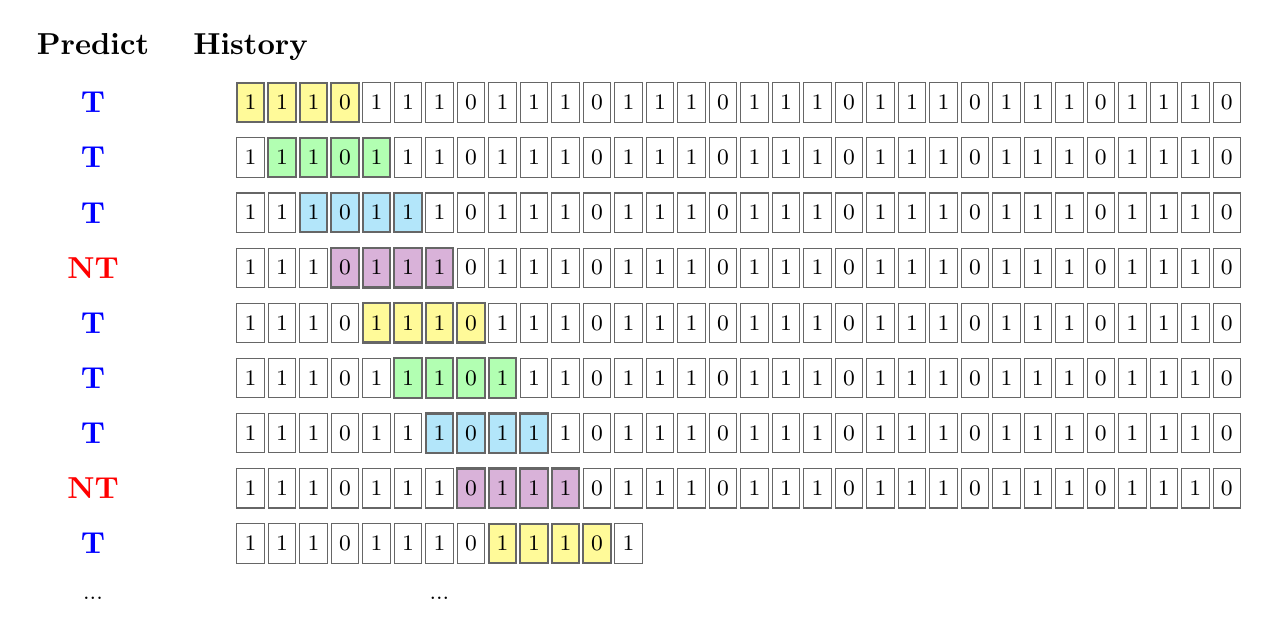
\begin{tikzpicture}[
    every node/.style={font=\footnotesize},
    bit/.style={minimum width=0.35cm, minimum height=0.5cm, inner sep=1pt, draw=black!60},
    history1110/.style={bit, fill=yellow!40, thick},
    history1101/.style={bit, fill=green!30, thick},
    history1011/.style={bit, fill=cyan!30, thick},
    history0111/.style={bit, fill=violet!30, thick},
    predict/.style={font=\fontsize{11}{13}\selectfont\bfseries, minimum width=1cm},
    label/.style={font=\fontsize{11}{13}\selectfont\bfseries}
]

% Labels positioned using relative positioning
\node[label, text height=1.5ex, text depth=.25ex] (predict_label) at (0, 0) {Predict};
\node[label, text height=1.5ex, text depth=.25ex] (history_label) at (2, 0) {History};

% Pattern template (repeated pattern: 11101110...)
\def\patternseq{1,1,1,0,1,1,1,0,1,1,1,0,1,1,1,0,1,1,1,0,1,1,1,0,1,1,1,0,1,1,1,0}

% Define row spacing
\def\rowspacing{0.7}

% Row 1 - History: 1110 -> Predict T
\node[predict, text=blue] (pred1) at (0, -1*\rowspacing) {T};
\foreach \i in {0,...,31} {
    \pgfmathparse{{\patternseq}[\i]}
    \pgfmathtruncatemacro{\val}{\pgfmathresult}
    \ifnum\i<4
        \node[history1110] at (2 + \i*0.4, -1*\rowspacing) {\val};
    \else
        \node[bit] at (2 + \i*0.4, -1*\rowspacing) {\val};
    \fi
}

% Row 2 - History: 1101 -> Predict T
\node[predict, text=blue] (pred2) at (0, -2*\rowspacing) {T};
\foreach \i in {0,...,31} {
    \pgfmathparse{{\patternseq}[\i]}
    \pgfmathtruncatemacro{\val}{\pgfmathresult}
    \ifnum\i>0 \ifnum\i<5
        \node[history1101] at (2 + \i*0.4, -2*\rowspacing) {\val};
    \else
        \node[bit] at (2 + \i*0.4, -2*\rowspacing) {\val};
    \fi \fi
    \ifnum\i=0
        \node[bit] at (2 + \i*0.4, -2*\rowspacing) {\val};
    \fi
}

% Row 3 - History: 1011 -> Predict T  
\node[predict, text=blue] (pred3) at (0, -3*\rowspacing) {T};
\foreach \i in {0,...,31} {
    \pgfmathparse{{\patternseq}[\i]}
    \pgfmathtruncatemacro{\val}{\pgfmathresult}
    \ifnum\i>1 \ifnum\i<6
        \node[history1011] at (2 + \i*0.4, -3*\rowspacing) {\val};
    \else
        \node[bit] at (2 + \i*0.4, -3*\rowspacing) {\val};
    \fi \fi
    \ifnum\i<2
        \node[bit] at (2 + \i*0.4, -3*\rowspacing) {\val};
    \fi
}

% Row 4 - History: 0111 -> Predict NT
\node[predict, text=red] (pred4) at (0, -4*\rowspacing) {NT};
\foreach \i in {0,...,31} {
    \pgfmathparse{{\patternseq}[\i]}
    \pgfmathtruncatemacro{\val}{\pgfmathresult}
    \ifnum\i>2 \ifnum\i<7
        \node[history0111] at (2 + \i*0.4, -4*\rowspacing) {\val};
    \else
        \node[bit] at (2 + \i*0.4, -4*\rowspacing) {\val};
    \fi \fi
    \ifnum\i<3
        \node[bit] at (2 + \i*0.4, -4*\rowspacing) {\val};
    \fi
}

% Row 5 - History: 1110 -> Predict T
\node[predict, text=blue] (pred5) at (0, -5*\rowspacing) {T};
\foreach \i in {0,...,31} {
    \pgfmathparse{{\patternseq}[\i]}
    \pgfmathtruncatemacro{\val}{\pgfmathresult}
    \ifnum\i>3 \ifnum\i<8
        \node[history1110] at (2 + \i*0.4, -5*\rowspacing) {\val};
    \else
        \node[bit] at (2 + \i*0.4, -5*\rowspacing) {\val};
    \fi \fi
    \ifnum\i<4
        \node[bit] at (2 + \i*0.4, -5*\rowspacing) {\val};
    \fi
}

% Row 6 - History: 1101 -> Predict T
\node[predict, text=blue] (pred6) at (0, -6*\rowspacing) {T};
\foreach \i in {0,...,31} {
    \pgfmathparse{{\patternseq}[\i]}
    \pgfmathtruncatemacro{\val}{\pgfmathresult}
    \ifnum\i>4 \ifnum\i<9
        \node[history1101] at (2 + \i*0.4, -6*\rowspacing) {\val};
    \else
        \node[bit] at (2 + \i*0.4, -6*\rowspacing) {\val};
    \fi \fi
    \ifnum\i<5
        \node[bit] at (2 + \i*0.4, -6*\rowspacing) {\val};
    \fi
}

% Row 7 - History: 1011 -> Predict T
\node[predict, text=blue] (pred7) at (0, -7*\rowspacing) {T};
\foreach \i in {0,...,31} {
    \pgfmathparse{{\patternseq}[\i]}
    \pgfmathtruncatemacro{\val}{\pgfmathresult}
    \ifnum\i>5 \ifnum\i<10
        \node[history1011] at (2 + \i*0.4, -7*\rowspacing) {\val};
    \else
        \node[bit] at (2 + \i*0.4, -7*\rowspacing) {\val};
    \fi \fi
    \ifnum\i<6
        \node[bit] at (2 + \i*0.4, -7*\rowspacing) {\val};
    \fi
}

% Row 8 - History: 0111 -> Predict NT
\node[predict, text=red] (pred8) at (0, -8*\rowspacing) {NT};
\foreach \i in {0,...,31} {
    \pgfmathparse{{\patternseq}[\i]}
    \pgfmathtruncatemacro{\val}{\pgfmathresult}
    \ifnum\i>6 \ifnum\i<11
        \node[history0111] at (2 + \i*0.4, -8*\rowspacing) {\val};
    \else
        \node[bit] at (2 + \i*0.4, -8*\rowspacing) {\val};
    \fi \fi
    \ifnum\i<7
        \node[bit] at (2 + \i*0.4, -8*\rowspacing) {\val};
    \fi
}

% Row 9 - History: 1110 -> Predict T
\node[predict, text=blue] (pred9) at (0, -9*\rowspacing) {T};
\foreach \i in {0,...,12} {
    \pgfmathparse{{\patternseq}[\i]}
    \pgfmathtruncatemacro{\val}{\pgfmathresult}
    \ifnum\i>7 \ifnum\i<12
        \node[history1110] at (2 + \i*0.4, -9*\rowspacing) {\val};
    \else
        \node[bit] at (2 + \i*0.4, -9*\rowspacing) {\val};
    \fi \fi
    \ifnum\i<8
        \node[bit] at (2 + \i*0.4, -9*\rowspacing) {\val};
    \fi
}

% ... dots
\node at (0, -10*\rowspacing) {...};
\node at (2 + 6*0.4, -10*\rowspacing) {...};

\end{tikzpicture}

\end{frame}

%==========================================
\definecolor{correctgreen}{RGB}{0,150,0}
\definecolor{incorrectred}{RGB}{200,0,0}
\definecolor{counterblue}{RGB}{70,130,255}
\definecolor{highlightyellow}{RGB}{255,230,100}
\definecolor{codeblue}{RGB}{0,0,200}

% Command to highlight state changes
\newcommand{\stateHighlight}[2]{%
  \ifnum#1=1
    \cellcolor{highlightyellow}#2%
  \else
    #2%
  \fi
}

% Macro for BHR display as boxes
\newcommand{\BHRbox}[4]{%
  \begin{tikzpicture}[baseline=(current bounding box.center)]
    \foreach \bit [count=\i] in {#1,#2,#3,#4} {
      \node[draw, minimum width=6mm, minimum height=5mm, inner sep=1pt] at (\i*0.7,0) {\footnotesize\bit};
    }
  \end{tikzpicture}
}

% Helper to expand stored BHR and pass to BHRbox
\newcommand{\BHRboxFromStorage}[4]{%
  % Direct storage of 4 values
  \BHRbox{#1}{#2}{#3}{#4}%
}

% Helper for pgfkeys stored BHR
\newcommand{\BHRdisplay}[1]{%
  % #1 contains {b1}{b2}{b3}{b4}
  % We need to extract these values
  \expandafter\BHRdisplayHelper#1%
}
\newcommand{\BHRdisplayHelper}[4]{%
  \BHRbox{#1}{#2}{#3}{#4}%
}

% Setup pgfkeys for local frame parameters
\pgfkeys{
  /localframe/.cd,
  ip/.store in=\localframeIP,
  ip/.default={},
  outcome/.store in=\localframeOutcome,
  bhr1/.code={\def\localframeBHROne{#1}},
  bhr2/.code={\def\localframeBHRTwo{#1}},
  bhr3/.code={\def\localframeBHRThree{#1}},
  r1/.store in=\localframeROne,
  r2/.store in=\localframeRTwo,
  r3/.store in=\localframeRThree,
  states/.store in=\localframeStates,
  description/.store in=\localframeDesc,
  % Set defaults - don't set BHR defaults, they cause issues
  ip={},
  outcome={},
  % bhr1={0}{0}{0}{0},  % Don't set default
  % bhr2={0}{0}{0}{0},  % Don't set default
  % bhr3={0}{0}{0}{0},  % Don't set default
  r1={0},
  r2={0},
  r3={0},
  states={},
  description={},
}
%==========================================
% Slide: 2-Level Branch Prediction
\begin{frame}
  \frametitle{2-Level Branch Prediction}

  \begin{itemize}
    \item 2-Level predictor uses \textbf{two levels}: a set of \textbf{Histories} and a set of \textbf{State machines}
    \item Instead of one state machine per branch, we maintain \textbf{2$^n$ state machines} (one for each possible history of $n$ bits)
    \item Select state machine based on the $n$ most recent branch outcomes (taken/not-taken)
    \item Each history pattern gets its own predictor
  \end{itemize}

  \vspace{1em}
  \begin{center}
    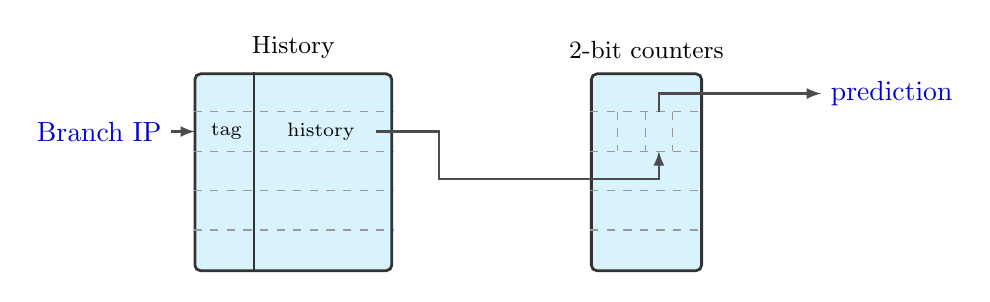
\begin{tikzpicture}[
      box/.style={draw=black!80, line width=1pt, minimum height=1cm, minimum width=2.5cm, fill=cyan!15, rounded corners=2pt, font=\small},
      bigbox/.style={draw=black!80, line width=1pt, fill=cyan!15, rounded corners=2pt},
      arrow/.style={-latex, thick, draw=black!70}
    ]

      % History cache with dashed rows - using relative positioning
      \node[bigbox, minimum width=2.5cm, minimum height=2.5cm] (hist_cache) at (3, 0) {};
      \node[above=0.05cm of hist_cache.north, font=\small] {History};

      % Draw vertical separator line for tag and history columns
      \draw[draw=black!80, line width=1pt] ([xshift=-0.5cm]hist_cache.north) -- ([xshift=-0.5cm]hist_cache.south);

      % Define row height to ensure consistency
      \def\rowheight{0.5cm}

      % Draw horizontal dashed lines for rows (5 rows total)
      \foreach \i in {1,2,3,4} {
        \draw[dashed, black!40] ([yshift=-\i*\rowheight]hist_cache.north west) -- ([yshift=-\i*\rowheight]hist_cache.north east);
      }

      % Define coordinates for tag and history boxes (2nd row)
      \coordinate (tag_box) at ([xshift=-0.85cm, yshift=-0.75cm]hist_cache.north);
      \coordinate (history_box) at ([xshift=0.35cm, yshift=-0.75cm]hist_cache.north);

      % Add labels in one of the rows (second row)
      \node[font=\scriptsize] at (tag_box) {tag};
      \node[font=\scriptsize] at (history_box) {history};

      % Define tag box west side for Branch IP positioning
      \coordinate (tag_west) at ([xshift=-1.25cm, yshift=-0.75cm]hist_cache.north);

      % Branch IP - anchored east, positioned relative to tag west
      \node[anchor=east, left=0.3cm of tag_west, font=\normalsize, text=blue!80!black] (ip) {Branch IP};

      % 2-bit counters array - using relative positioning, 2x wider
      \def\counterwidth{1.4cm}

      % Draw outer box for counter array to match history table height
      \node[bigbox, minimum width=\counterwidth, minimum height=2.5cm, right=2.5cm of hist_cache] (counter_array) {};
      \node[above=0.05cm of counter_array.north, font=\small] {2-bit counters};

      % Draw horizontal dashed lines for counter array rows
      \foreach \i in {1,2,3,4} {
        \draw[dashed, black!40] ([yshift=-\i*\rowheight]counter_array.north west) -- ([yshift=-\i*\rowheight]counter_array.north east);
      }

      % Draw vertical dashed lines in 2nd row to show array elements
      % 2nd row spans from yshift=-0.5cm to yshift=-1.0cm (between 1st and 2nd dashed horizontal lines)
      \def\numelements{4}
      \coordinate (row2_top) at ([yshift=-0.5cm]counter_array.north west);
      \coordinate (row2_bottom) at ([yshift=-1.0cm]counter_array.north west);

      \foreach \i in {1,2,3} {
        \pgfmathsetmacro{\xpos}{\i*\counterwidth/\numelements}
        \draw[dashed, black!40] ([xshift=\xpos]row2_top) -- ([xshift=\xpos]row2_bottom);
      }

      % Define the 3rd array element positions in 2nd row
      \pgfmathsetmacro{\thirdelem}{2.5*\counterwidth/\numelements}
      \coordinate (third_element_top) at ([xshift=\thirdelem, yshift=-0.5cm]counter_array.north west);
      \coordinate (third_element_bottom) at ([xshift=\thirdelem, yshift=-1.0cm]counter_array.north west);

      % Prediction output - positioned higher with yshift
      \node[anchor=west, right=1.5cm of counter_array.east, yshift=1cm, font=\normalsize, text=blue!80!black] (prediction) {prediction};

      % Arrows
      \draw[arrow] (ip) -- (tag_west);

      % Arrow from history: go right, then up, then use -| to south of 3rd element
      \draw[arrow] ([xshift=0.7cm]history_box) -- ++(0.8, 0) -- ++(0, -0.6) -| (third_element_bottom);

      % Arrow from top of 3rd element to prediction
      \draw[arrow] (third_element_top) |- (prediction.west);

    \end{tikzpicture}
  \end{center}
\end{frame}

%==========================================
% Slide: Branch History Register (BHR)
\begin{frame}
  \frametitle{Branch History Register (BHR): Shift Register Mechanism}

  \begin{itemize}
    \item A \textbf{shift register} of $n$ bits tracks branch history at every moment
    \item Each bit represents: \textbf{0} = not-taken, \textbf{1} = taken
    \item Example: BHR with length 5 bits
  \end{itemize}

  \vspace{1em}
  \begin{center}
    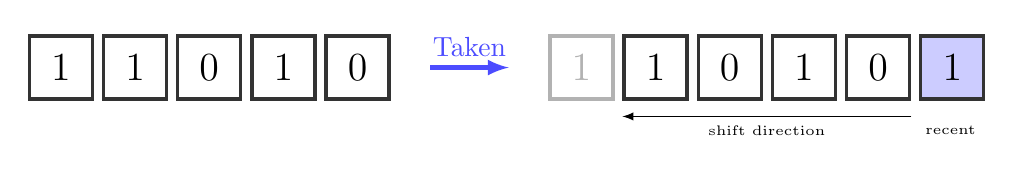
\begin{tikzpicture}[
      box/.style={draw=black!80, line width=1.2pt, minimum width=0.8cm, minimum height=0.8cm, font=\Large},
      fadedbox/.style={draw=black!30, line width=1.2pt, minimum width=0.8cm, minimum height=0.8cm, font=\Large, text=black!30}
    ]
      % First BHR state
      \node[box] (box0) at (0, 0) {1};
      \node[box, anchor=west] (box1) at ([xshift=1mm]box0.east) {1};
      \node[box, anchor=west] (box2) at ([xshift=1mm]box1.east)  {0};
      \node[box, anchor=west] (box3) at ([xshift=1mm]box2.east)  {1};
      \node[box, anchor=west] (box4) at ([xshift=1mm]box3.east)  {0};

      % Faded evicted bit on the left - relative positioning
      \node[fadedbox, anchor=west] (evicted) at ([xshift=2cm]box4.east) {1};

      % Second BHR state after taken - relative to evicted box
      \node[box, anchor=west] (newbox0) at ([xshift=1mm]evicted.east) {1};
      \node[box, anchor=west] (newbox1) at ([xshift=1mm]newbox0.east) {0};
      \node[box, anchor=west] (newbox2) at ([xshift=1mm]newbox1.east) {1};
      \node[box, anchor=west] (newbox3) at ([xshift=1mm]newbox2.east) {0};
      \node[box, fill=blue!20, anchor=west] (newbox4) at ([xshift=1mm]newbox3.east) {1};

      % Arrow showing transition - relative to box4
      \draw[-latex, ultra thick, blue!70] ([xshift=5mm]box4.east) -- ([xshift=-5mm]evicted.west) node[midway, above] {Taken};

      % Arrow showing shift direction (left-pointing) between boxes
      \draw[-latex] ([yshift=-2mm]newbox3.south east) -- ([yshift=-2mm]newbox0.south west) node[midway, below, font=\tiny] {shift direction};

      % "recent" label aligned to rightmost box
      \node[anchor=north east, font=\tiny] (recent) at ([yshift=-2mm]newbox4.south east) {recent};



    \end{tikzpicture}
  \end{center}

  \vspace{2em}
  \begin{tcolorbox}[colback=blue!10, colframe=blue!50]
    \small
    \textbf{Shift operation:} New result enters from the \textbf{right} (most recent), register shifts left, oldest bit is \textbf{discarded} from the left
  \end{tcolorbox}
\end{frame}

%==========================================
% Slide: Local vs Global BHR
\begin{frame}[fragile]
  \frametitle{BHR Types: Local vs Global}

  \vspace{-0.3cm}
  \begin{columns}[t]
    \column{0.48\textwidth}
    \textbf{\large Local BHR}
    \vspace{0.3em}
    \begin{itemize}
      \item Each branch instruction has its own BHR (local BHR)
      \item Effective for capturing recurring patterns of a specific branch
    \end{itemize}

    \textbf{Example:}
    \begin{tcolorbox}[colback=green!5, colframe=green!40, boxrule=0.8pt]
      \small
\begin{verbatim}
for (j=0; j<4; j++)
  { ... }
\end{verbatim}
      \vspace{-0.5em}
      Pattern: \texttt{1110}\\
      Local BHR captures this pattern
    \end{tcolorbox}

    \column{0.48\textwidth}
    \textbf{\large Global BHR}
    \vspace{0.3em}
    \begin{itemize}
      \item One shared global History Register for all Branch instructions
      \item Effective for capturing dependencies between different branches
    \end{itemize}

    \textbf{Example:}
    \begin{tcolorbox}[colback=blue!5, colframe=blue!40, boxrule=0.8pt]
      \small
\begin{verbatim}
if (...)
  if (...)
    if (...)
      if (true) { ... }
\end{verbatim}
      \vspace{-0.5em}
      When global history is \texttt{111}, always predict Taken
    \end{tcolorbox}
  \end{columns}
\end{frame}

%==========================================
% Slide: Prediction State Machine Table
\begin{frame}
  \frametitle{Prediction State Machine Table}

  \begin{columns}[t]
    \column{0.48\textwidth}
    \textbf{\large Local (Per Branch) Table}
    \vspace{0.1em}
    \begin{itemize}
      \item Can hold a separate (local) state machine table for each branch instruction
    \end{itemize}

    \column{0.48\textwidth}
    \textbf{\large Global Table}
    \vspace{0.1em}
    \begin{itemize}
      \item Can hold a global state machine table to save space
      \item Allows longer BHRs (note that the table grows exponentially)
    \end{itemize}
  \end{columns}

  \vspace{-0.8em}
  \begin{columns}[t]
    \column{0.48\textwidth}
    \begin{tcolorbox}[colback=green!5, colframe=green!40, boxrule=0.8pt, height=3.2cm]
      \footnotesize
      \textbf{Dedicated} per branch\\[0.3em]
      \textbf{Accuracy:} {\color{green!70!black}\checkmark} More accurate\\[0.3em]
      \textbf{Space:} {\color{red!70!black}\texttimes} Uses more space\\[0.3em]
      \textbf{Size:} $M \times 2^n$ counters\\
      \hspace*{1em}($M$ branches, $n$ = history length)
    \end{tcolorbox}

    \column{0.48\textwidth}
    \begin{tcolorbox}[colback=blue!5, colframe=blue!40, boxrule=0.8pt, height=3.2cm]
      \footnotesize
      \textbf{Shared} by all branches\\[0.3em]
      \textbf{Accuracy:} {\color{red!70!black}\texttimes} May have conflicts\\[0.3em]
      \textbf{Space:} {\color{green!70!black}\checkmark} Saves space\\[0.3em]
      \textbf{Size:} $2^n$ counters total\\
      \hspace*{1em}($n$ = history length)
    \end{tcolorbox}
  \end{columns}

  \vspace{-0.1em}
  \begin{tcolorbox}[colback=orange!10, colframe=orange!50]
    \centering
    \textbf{Trade-off:} Accuracy vs Space
  \end{tcolorbox}
\end{frame}

%==========================================
% Slide: Local BHR Table and Size Calculation
\begin{frame}
  \frametitle{Local BHR Table and Size (Question)}

  \textbf{Example:} Calculate predictor size for the following configuration:

  \vspace{0.3em}
  \begin{columns}[t]
    \column{0.48\textwidth}
    \textbf{Address Format:}
    \begin{itemize}
      \item 32-bit addresses
      \item 4-byte aligned instructions
    \end{itemize}
    \vspace{0.3em}
    \centering
    \addressbreakdown{30}{0}{2}

    \column{0.48\textwidth}
    \textbf{History Table:}
    \begin{itemize}
      \item 1024 entries
      \item Fully associative
      \item History length: 4 bits
    \end{itemize}
  \end{columns}

  \vspace{0.3em}
  \textbf{What is the predictor size?}

  \pause
  \vspace{-0.2em}
  \begin{tcolorbox}[colback=blue!10, colframe=blue!50, title=Formula]
    \small
    \textbf{Predictor size} = \#entries $\times$ (tag\_size + history\_size + $2 \times 2^{\text{history\_size}}$)
  \end{tcolorbox}

  \pause
  \vspace{-0.8em}
  \begin{tcolorbox}[colback=green!10, colframe=green!50]
    \centering
    \textbf{Predictor size} = $1024 \times (30 + 4 + 2 \times 2^4) = 1024 \times 66 = \textbf{66 Kbits}$
  \end{tcolorbox}
\end{frame}

%==========================================
\begin{frame}
  \frametitle{Code Example}
  
  \begin{columns}[T]
    \column{0.42\textwidth}
    \centering
    \textbf{C Code}
    \vspace{0.5em}
    
    \begin{tcolorbox}[colback=white, colframe=black!60, boxrule=0.8pt, left=3pt, right=3pt, top=3pt, bottom=3pt]
      \small\ttfamily
      \begin{tabbing}
      \hspace{1em}\=\hspace{1em}\=\kill
      \colorbox{red!25}{for (i=100; i>0; i--)}\\ 
      \> \colorbox{green!25}{for (j=2; j<5; j++)}\\
      \> \> \colorbox{cyan!25}{if (i\%j == 0)} \{\\
      \> \>   \colorbox{gray!15}{. . .}\\
      \> \> \}\\
      \end{tabbing}
    \end{tcolorbox}
    
    \column{0.58\textwidth}
    \centering
    \textbf{Assembly}
    \vspace{0.5em}
    
    \begin{tcolorbox}[colback=white, colframe=black!60, boxrule=0.8pt, left=3pt, right=3pt, top=3pt, bottom=3pt]
      \small\ttfamily
      \renewcommand{\arraystretch}{1.1}
      \begin{tabular}{@{}r@{~~}l@{}}
        & \colorbox{green!25}{Addi~~~r5, r0, 5}\\
        & \colorbox{red!25}{Addi~~~r1, r0, 100}\\
        L1: & \colorbox{green!25}{Addi~~~r2, r0, 2}\\
        L2: & \colorbox{cyan!25}{Mod~~~~r3, r1, r2}\\
        & \colorbox{cyan!25}{Bne~~~~r3, r0, IF}\\
        & \colorbox{gray!15}{. . .}\\
        IF: & \colorbox{green!25}{Addi~~~r2, r2, 1}\\
        & \colorbox{green!25}{Bne~~~~r2, r5, L2}\\
        & \colorbox{red!25}{Subi~~~r1, r1, 1}\\
        & \colorbox{red!25}{Bne~~~~r1, r0, L1}\\
      \end{tabular}
    \end{tcolorbox}
  \end{columns}
  
  \vspace{0.8em}
  
  \begin{center}
    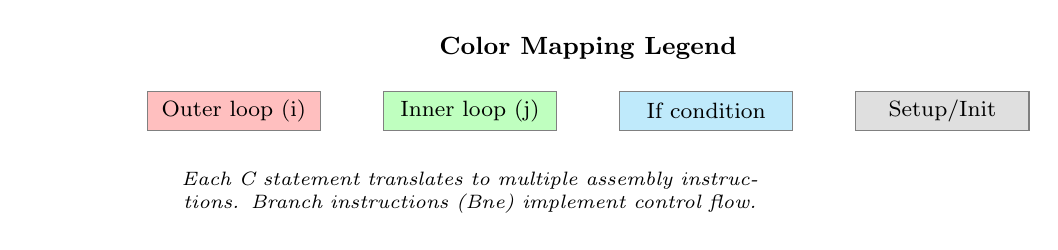
\begin{tikzpicture}[
      legend/.style={draw=black!50, minimum width=2.2cm, minimum height=0.5cm, font=\footnotesize, inner sep=2pt}
    ]
      % Legend title
      \node[font=\small\bfseries] at (0, 0.8) {Color Mapping Legend};
      
      % Legend boxes
      \node[legend, fill=red!25] (outer) at (-4.5,0) {Outer loop (i)};
      \node[legend, fill=green!25] (inner) at (-1.5,0) {Inner loop (j)};
      \node[legend, fill=cyan!25] (if) at (1.5,0) {If condition};
      \node[legend, fill=gray!25] (init) at (4.5,0) {Setup/Init};
      
      % Note
      \node[below=0.4cm of inner, font=\scriptsize\itshape, text width=11cm, align=center] {
        Each C statement translates to multiple assembly instructions. Branch instructions (Bne) implement control flow.
      };
    \end{tikzpicture}
  \end{center}
\end{frame}

% New local frame macro using pgfkeys
\newcommand{\localFrameKV}[1]{%
  % Initialize BHR variables to defaults
  \def\localframeBHROne{{0}{0}{0}{0}}%
  \def\localframeBHRTwo{{0}{0}{0}{0}}%
  \def\localframeBHRThree{{0}{0}{0}{0}}%
  \pgfkeys{/localframe/.cd,#1}%
  \begin{frame}
    \frametitle{Local History Branch Predictor}
    \begin{columns}[T]
      \column{0.30\textwidth}
      \begin{tcolorbox}[colback=gray!5, colframe=gray!50, boxrule=0.5pt, left=2pt, right=2pt, top=2pt, bottom=2pt]
        \footnotesize\ttfamily
        \begin{tabbing}
        \hspace{2em}\=\hspace{2em}\=\kill
        \> Addi r5, r0, 5\\
        \> Addi r1, r0, 100\\
        L1:\> Addi r2, r0, 2\\
        L2:\> Mod r3, r1, r2\\
        \ifnum\pdfstrcmp{\localframeIP}{IP1}=0
          \>\colorbox{highlightyellow}{Bne r3, r0, IF} \hspace{-1em}\textcolor{red}{$\leftarrow$ \textbf{PC}}\\
        \else
          \> Bne r3, r0, IF\\
        \fi
        \> . . .\\
        IF:\> Addi r2, r2, 1\\
        \ifnum\pdfstrcmp{\localframeIP}{IP2}=0
          \>\colorbox{highlightyellow}{Bne r2, r5, L2} \hspace{-1em}\textcolor{red}{$\leftarrow$ \textbf{PC}}\\
        \else
          \> Bne r2, r5, L2\\
        \fi
        \> Subi r1, r1, 1\\
        \ifnum\pdfstrcmp{\localframeIP}{IP3}=0
          \>\colorbox{highlightyellow}{Bne r1, r0, L1} \hspace{-1em}\textcolor{red}{$\leftarrow$ \textbf{PC}}\\
        \else
          \> Bne r1, r0, L1\\
        \fi
        \end{tabbing}
      \end{tcolorbox}
      \centering
      \colorbox{highlightyellow}{\textbf{\localframeOutcome}}
      
     
    \column{0.35\textwidth}
      \centering

      \footnotesize
      \begin{tabular}{|c|ccc|c}
          \toprule
          tag & \multicolumn{4}{c|}{BHRs} \\
          \midrule
          \ifnum\pdfstrcmp{\localframeIP}{IP1}=0
            \cellcolor{highlightyellow}IP1 & \multicolumn{4}{c|}{\BHRdisplay{\localframeBHROne}} \\
          \else
            IP1 & \multicolumn{4}{c|}{\BHRdisplay{\localframeBHROne}} \\
          \fi
          \ifnum\pdfstrcmp{\localframeIP}{IP2}=0
            \cellcolor{highlightyellow}IP2 & \multicolumn{4}{c|}{\BHRdisplay{\localframeBHRTwo}} \\
          \else
            IP2 & \multicolumn{4}{c|}{\BHRdisplay{\localframeBHRTwo}} \\
          \fi
          \ifnum\pdfstrcmp{\localframeIP}{IP3}=0
            \cellcolor{highlightyellow}IP3 & \multicolumn{4}{c|}{\BHRdisplay{\localframeBHRThree}} \\
          \else
            IP3 & \multicolumn{4}{c|}{\BHRdisplay{\localframeBHRThree}} \\
          \fi
          \bottomrule
      \end{tabular}
      
      \vspace{0.8em}
          \centering
          \begin{tabular}{|c|r|}
          \toprule
          Reg & Value \\
          \midrule
          r1 & \localframeROne \\
          r2 & \localframeRTwo \\
          r3 & \localframeRThree \\
          \bottomrule
          \end{tabular}
          
    \column{0.35\textwidth}
      \centering\scriptsize
      \stateTable{\localframeStates}
      
      \vspace{0.5em}
      \centering
    \end{columns}
    \vspace{0.5em}
    \centering
    \textcolor{blue}{\small \localframeDesc}
  \end{frame}
}

% Wrapper for old localFrame calls - converts to key-value format
\newcommand{\localFrame}[9]{%
  \localFrameKV{
    outcome={#1},
    bhr1={#2},
    bhr2={#3},
    bhr3={#4},
    r1={#5},
    r2={#6},
    r3={#7},
    states={#8},
    description={#9}
  }
}

% Setup pgfkeys for global frame parameters
\pgfkeys{
  /globalframe/.cd,
  ip/.store in=\globalframeIP,
  ip/.default={},
  outcome/.store in=\globalframeOutcome,
  bhr/.code={\def\globalframeBHR{#1}},
  r1/.store in=\globalframeROne,
  r2/.store in=\globalframeRTwo,
  r3/.store in=\globalframeRThree,
  states/.store in=\globalframeStates,
  description/.store in=\globalframeDesc,
  % Set defaults - don't set BHR default
  ip={},
  outcome={},
  % bhr={0}{0}{0}{0},  % Don't set default
  r1={0},
  r2={0},
  r3={0},
  states={},
  description={},
}

% New global frame macro using pgfkeys
\newcommand{\globalFrameKV}[1]{%
  % Initialize BHR variable to default
  \def\globalframeBHR{{0}{0}{0}{0}}%
  \pgfkeys{/globalframe/.cd,#1}%
  \begin{frame}
    \frametitle{Global History Branch Predictor}
    \begin{columns}[T]
      \column{0.30\textwidth}
      \begin{tcolorbox}[colback=gray!5, colframe=gray!50, boxrule=0.5pt, left=2pt, right=2pt, top=2pt, bottom=2pt]
        \footnotesize\ttfamily
        \begin{tabbing}
        \hspace{2em}\=\hspace{2em}\=\kill
        \> Addi r5, r0, 5\\
        \> Addi r1, r0, 100\\
        L1:\> Addi r2, r0, 2\\
        L2:\> Mod r3, r1, r2\\
        \ifnum\pdfstrcmp{\globalframeIP}{IP1}=0
          \>\colorbox{highlightyellow}{Bne r3, r0, IF} \hspace{-1em}\textcolor{red}{$\leftarrow$ \textbf{PC}}\\
        \else
          \> Bne r3, r0, IF\\
        \fi
        \> . . .\\
        IF:\> Addi r2, r2, 1\\
        \ifnum\pdfstrcmp{\globalframeIP}{IP2}=0
          \>\colorbox{highlightyellow}{Bne r2, r5, L2} \hspace{-1em}\textcolor{red}{$\leftarrow$ \textbf{PC}}\\
        \else
          \> Bne r2, r5, L2\\
        \fi
        \> Subi r1, r1, 1\\
        \ifnum\pdfstrcmp{\globalframeIP}{IP3}=0
          \>\colorbox{highlightyellow}{Bne r1, r0, L1} \hspace{-1em}\textcolor{red}{$\leftarrow$ \textbf{PC}}\\
        \else
          \> Bne r1, r0, L1\\
        \fi
        \end{tabbing}
      \end{tcolorbox}
      
      \vspace{0.5em}
      \centering
      \colorbox{highlightyellow}{\textbf{\globalframeOutcome}}
      
      \column{0.35\textwidth}
      \centering
      \footnotesize
      \textbf{Global BHR}\\[0.3em]
      \BHRdisplay{\globalframeBHR}
      
      \vspace{0.8em}
      \begin{tabular}{|c|r|}
        \toprule
        Reg & Value \\
        \midrule
        r1 & \globalframeROne \\
        r2 & \globalframeRTwo \\
        r3 & \globalframeRThree \\
        \bottomrule
      \end{tabular}
      
      \vspace{0.5em}
     
      \column{0.35\textwidth}
      \centering
      \footnotesize
      \textbf{Global Table}\\[0.3em]
      \scriptsize
      \stateTable{\globalframeStates}
    \end{columns}
      \centering
      \textcolor{blue}{\small \globalframeDesc}
   \end{frame}
}

% Wrapper for old globalFrame calls - converts to key-value format
\newcommand{\globalFrame}[7]{%
  \globalFrameKV{
    outcome={#1},
    bhr={#2},
    r1={#3},
    r2={#4},
    r3={#5},
    states={#6},
    description={#7}
  }
}

% State table macro
\newcommand{\stateTable}[1]{%
  % #1: comma-separated list of index:state:highlight
  % Format: 0:WT:0,3:ST:1,12:WNT:0,...
  \begin{tabular}{|c|c|}
    \toprule
    \multicolumn{2}{|c|}{States} \\
    \midrule
    \stateRow{0}{#1} \\
    \stateRow{1}{#1} \\
    \stateRow{2}{#1} \\
    \stateRow{3}{#1} \\
    \stateRow{4}{#1} \\
    \stateRow{5}{#1} \\
    \stateRow{6}{#1} \\
    \stateRow{7}{#1} \\
    \stateRow{8}{#1} \\
    \stateRow{9}{#1} \\
    \stateRow{10}{#1} \\
    \stateRow{11}{#1} \\
    \stateRow{12}{#1} \\
    \stateRow{13}{#1} \\
    \stateRow{14}{#1} \\
    \stateRow{15}{#1} \\
    \bottomrule
  \end{tabular}
}

% Helper to format state with color
\newcommand{\formatState}[1]{%
  \ifnum\pdfstrcmp{#1}{ST}=0\textcolor{correctgreen}{\textbf{#1}}%
  \else\ifnum\pdfstrcmp{#1}{WT}=0#1%
  \else\ifnum\pdfstrcmp{#1}{WNT}=0\textcolor{incorrectred}{#1}%
  \else\ifnum\pdfstrcmp{#1}{SNT}=0\textcolor{incorrectred}{\textbf{#1}}%
  \else #1%
  \fi\fi\fi\fi%
}

% Helper to get state for specific index
\newcommand{\stateRow}[2]{%
  % #1: index, #2: full state string
  % Returns the row for this index
  #1 & \getStateForIndex{#1}{#2}%
}

% Parse state string and return formatted state for given index
\newcommand{\getStateForIndex}[2]{%
  % Default all to WT, then override based on input
  \def\tempstate{WT}%
  \def\temphighlight{0}%
  % Parse the input string for this index
  \parseStateString{#1}{#2}%
  \ifnum\temphighlight=1
    \cellcolor{highlightyellow}\formatState{\tempstate}%
  \else
    \formatState{\tempstate}%
  \fi
}

% Helper to parse state string - simplified version
\newcommand{\parseStateString}[2]{%
  % This is a simplified implementation
  % In practice, you'd parse #2 to find if #1 appears
  % For now, using manual specification in frames
}

% Advanced macro for complete state specification
% Usage: \fullStateTable{index1/state1/highlight1,index2/state2/highlight2,...}
\newcommand{\fullStateTable}[1]{%
  \def\stateZero{WT}\def\highlightZero{0}%
  \def\stateOne{WT}\def\highlightOne{0}%
  \def\stateTwo{WT}\def\highlightTwo{0}%
  \def\stateThree{WT}\def\highlightThree{0}%
  \def\stateFour{WT}\def\highlightFour{0}%
  \def\stateFive{WT}\def\highlightFive{0}%
  \def\stateSix{WT}\def\highlightSix{0}%
  \def\stateSeven{WT}\def\highlightSeven{0}%
  \def\stateEight{WT}\def\highlightEight{0}%
  \def\stateNine{WT}\def\highlightNine{0}%
  \def\stateTen{WT}\def\highlightTen{0}%
  \def\stateEleven{WT}\def\highlightEleven{0}%
  \def\stateTwelve{WT}\def\highlightTwelve{0}%
  \def\stateThirteen{WT}\def\highlightThirteen{0}%
  \def\stateFourteen{WT}\def\highlightFourteen{0}%
  \def\stateFifteen{WT}\def\highlightFifteen{0}%
  % Parse input and update states
  % For demonstration, manually setting based on frame
  \begin{tabular}{c|c||c|c}
    \toprule
    \multicolumn{2}{c||}{States 0-7} & \multicolumn{2}{c}{States 8-15} \\
    \midrule
    0 & \ifnum\highlightZero=1\cellcolor{highlightyellow}\fi\formatState{\stateZero} & 
    8 & \ifnum\highlightEight=1\cellcolor{highlightyellow}\fi\formatState{\stateEight} \\
    1 & \ifnum\highlightOne=1\cellcolor{highlightyellow}\fi\formatState{\stateOne} & 
    9 & \ifnum\highlightNine=1\cellcolor{highlightyellow}\fi\formatState{\stateNine} \\
    2 & \ifnum\highlightTwo=1\cellcolor{highlightyellow}\fi\formatState{\stateTwo} & 
    10 & \ifnum\highlightTen=1\cellcolor{highlightyellow}\fi\formatState{\stateTen} \\
    3 & \ifnum\highlightThree=1\cellcolor{highlightyellow}\fi\formatState{\stateThree} & 
    11 & \ifnum\highlightEleven=1\cellcolor{highlightyellow}\fi\formatState{\stateEleven} \\
    4 & \ifnum\highlightFour=1\cellcolor{highlightyellow}\fi\formatState{\stateFour} & 
    12 & \ifnum\highlightTwelve=1\cellcolor{highlightyellow}\fi\formatState{\stateTwelve} \\
    5 & \ifnum\highlightFive=1\cellcolor{highlightyellow}\fi\formatState{\stateFive} & 
    13 & \ifnum\highlightThirteen=1\cellcolor{highlightyellow}\fi\formatState{\stateThirteen} \\
    6 & \ifnum\highlightSix=1\cellcolor{highlightyellow}\fi\formatState{\stateSix} & 
    14 & \ifnum\highlightFourteen=1\cellcolor{highlightyellow}\fi\formatState{\stateFourteen} \\
    7 & \ifnum\highlightSeven=1\cellcolor{highlightyellow}\fi\formatState{\stateSeven} & 
    15 & \ifnum\highlightFifteen=1\cellcolor{highlightyellow}\fi\formatState{\stateFifteen} \\
    \bottomrule
  \end{tabular}
}

\section{Local History Branch Predictor}

% Local History Predictor Frames
\localFrameKV{
    ip={IP1},
    outcome={Not Taken},
    r1={100},
    r2={2},
    r3={0},
    bhr1={0}{0}{0}{0},
    bhr2={0}{0}{0}{0},
    bhr3={0}{0}{0}{0},
    states={0:WT:0},
    description={Initial state with IP1 highlighted}
  }

% localFrameKV call removed - causes brace errors even with BHR commented

% Comment out to isolate the error source
% \localFrame{Not Taken}{{0}{0}{0}{0}}{{0}{0}{0}{0}}{{0}{0}{0}{0}}{100}{2}{0}{0:WNT:1}{Misprediction (predicted taken, was not taken)}

% \localFrame{Taken}{{0}{0}{0}{0}}{{0}{0}{0}{0}}{{0}{0}{0}{0}}{100}{3}{0}{0:WT:1}{State update}

\localFrame{Taken}{{0}{0}{0}{0}}{{0}{0}{0}{1}}{{0}{0}{0}{0}}{100}{3}{0}{0:ST:1}{Correct prediction}

\localFrame{Taken}{{0}{0}{0}{0}}{{0}{0}{0}{1}}{{0}{0}{0}{0}}{100}{3}{1}{0:WNT:0}{State update}

\localFrame{Taken}{{0}{0}{0}{1}}{{0}{0}{0}{1}}{{0}{0}{0}{0}}{100}{3}{1}{0:WT:1}{Misprediction}

\localFrame{Taken}{{0}{0}{0}{1}}{{0}{0}{0}{1}}{{0}{0}{0}{0}}{100}{4}{1}{0:ST:1}{Correct prediction}

\localFrame{Taken}{{0}{0}{0}{1}}{{0}{0}{1}{1}}{{0}{0}{0}{0}}{100}{4}{1}{0:ST:1}{Correct prediction}

\localFrame{Not Taken}{{0}{0}{0}{1}}{{0}{0}{1}{1}}{{0}{0}{0}{0}}{100}{4}{0}{0:ST:0}{State update}

\localFrame{Not Taken}{{0}{0}{1}{0}}{{0}{0}{1}{1}}{{0}{0}{0}{0}}{100}{4}{0}{0:WNT:1}{Misprediction}

\localFrame{Not Taken}{{0}{0}{1}{0}}{{0}{0}{1}{1}}{{0}{0}{0}{0}}{100}{5}{0}{0:ST:1,3:ST:0}{State update}

\localFrame{Not Taken}{{0}{0}{1}{0}}{{0}{1}{1}{0}}{{0}{0}{0}{0}}{100}{5}{0}{3:WNT:1}{Misprediction}

\localFrame{Taken}{{0}{0}{1}{0}}{{0}{1}{1}{0}}{{0}{0}{0}{0}}{99}{5}{0}{0:ST:0}{State update}

\localFrame{Taken}{{0}{0}{1}{0}}{{0}{1}{1}{0}}{{0}{0}{0}{1}}{99}{5}{0}{0:ST:1}{Correct prediction}

% Transition slide
\begin{frame}
  \frametitle{Global History Predictor}
  \begin{center}
    \Large Now switching to \textbf{Global BHR}
  \end{center}

  \vspace{0.5em}

  \begin{itemize}
    \item Using a single global BHR table
    \item In contrast to local predictors (each IP has own BHR and state table)
    \item Still tracking history of 4 branches (4-bit BHR)
  \end{itemize}

  \vspace{0.5em}
  \textbf{What is the predictor size?}

  \pause
  \vspace{-0.1em}
  \begin{tcolorbox}[colback=blue!10, colframe=blue!50, title=Formula]
    \small
    \textbf{Predictor size} = history\_size + $2 \times 2^{\text{history\_size}}$
  \end{tcolorbox}

  \pause
  \vspace{-0.8em}
  \begin{tcolorbox}[colback=green!10, colframe=green!50]
    \centering
    \textbf{Predictor size} = $4 + 2 \times 2^4 = 4 + 32 = \textbf{36 bits}$\\[0.3em]
    \textcolor{correctgreen}{vs. 66 Kbits for local history/state arrays!}
  \end{tcolorbox}
\end{frame}

% Global History Predictor Frames
% Example with instruction pointer highlighting using pgfkeys
% For now, use the old syntax until we fix the pgfkeys issue
\globalFrame{Not Taken}{{0}{0}{0}{0}}{100}{2}{0}{0:WT:0}{Global BHR - Initial state}

\globalFrame{Not Taken}{{0}{0}{0}{0}}{100}{2}{0}{0:WNT:1}{Misprediction (predicted taken, was not taken)}

\globalFrame{Taken}{{0}{0}{0}{0}}{100}{3}{0}{0:WNT:0}{State update}

\globalFrame{Taken}{{0}{0}{0}{1}}{100}{3}{0}{0:WT:1}{Misprediction}

\globalFrame{Taken}{{0}{0}{0}{1}}{100}{3}{1}{0:WT:0}{State update}

\globalFrame{Taken}{{0}{0}{1}{1}}{100}{3}{1}{3:ST:1}{Correct prediction}

\globalFrame{Taken}{{0}{0}{1}{1}}{100}{4}{1}{3:ST:0}{State update}

\globalFrame{Taken}{{0}{1}{1}{1}}{100}{4}{1}{3:ST:1}{Correct prediction}

\globalFrame{Not Taken}{{0}{1}{1}{1}}{100}{4}{0}{3:ST:0}{State update}

\globalFrame{Not Taken}{{1}{1}{1}{0}}{100}{4}{0}{14:WNT:1}{Misprediction}

\globalFrame{Not Taken}{{1}{1}{1}{0}}{100}{5}{0}{14:WNT:0}{State update}

\globalFrame{Not Taken}{{1}{1}{0}{0}}{100}{5}{0}{12:WNT:1}{Misprediction}

\globalFrame{Taken}{{1}{1}{0}{0}}{99}{5}{0}{12:WT:0}{State update}

\globalFrame{Taken}{{1}{0}{0}{1}}{99}{5}{0}{12:ST:1}{Correct prediction}

%==========================================
% Add more slides here as needed

% Slide 1: Global Prediction Table Issues
\begin{frame}
  \frametitle{Global Prediction Table}
  
  \textbf{Problem:} Collision between different branch instructions in global tables
  
  \begin{itemize}
    \item Different branch instructions with the same (local) history at a given moment modify the same state machines:
    \begin{itemize}
      \item Branch 1: (IP = ...0101) History = 1101 → Taken
      \item Branch 2: (IP = ...1010) History = 1101 → Not Taken
    \end{itemize}
  \end{itemize}
  
  \vspace{0.5em}
  
  \textbf{Solution:} Create hashing in the table by XORing BHR with Branch IP
  \begin{itemize}
    \item Select state machine based on: BHR $\oplus$ Branch IP
    \begin{itemize}
      \item Branch 1: IP $\oplus$ History = 0101 $\oplus$ 1101 = 1000 → Taken
      \item Branch 2: IP $\oplus$ History = 1010 $\oplus$ 1101 = 0111 → Not Taken
    \end{itemize}
  \end{itemize}
  
  \vspace{0.5em}
  
  \begin{tcolorbox}[colback=blue!10, colframe=blue!50]
    \centering
    \textbf{This approach is called:}\\
    \textbf{L-Share} (Local BHR) or \textbf{G-Share} (Global BHR)\\
    \small Note: L-Share/G-Share refers to global state table only!
  \end{tcolorbox}
\end{frame}

% Slide 2: LShare Predictor Architecture
\begin{frame}
  \frametitle{Local Predictor: LShare}

  \begin{center}
    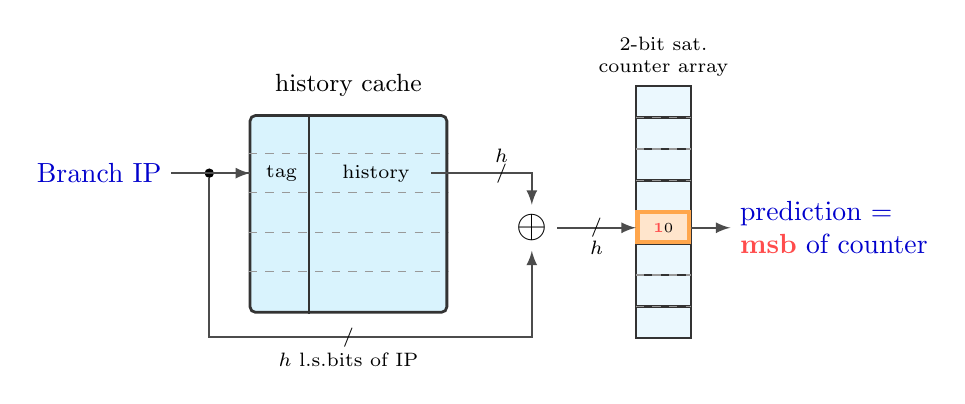
\begin{tikzpicture}[
      box/.style={draw=black!80, line width=1pt, minimum height=1cm, minimum width=2.5cm, fill=cyan!15, rounded corners=2pt, font=\small},
      bigbox/.style={draw=black!80, line width=1pt, fill=cyan!15, rounded corners=2pt},
      arrow/.style={-latex, thick, draw=black!70},
      data_connector/.style={circle, fill=black, inner sep=1.2pt}
    ]
      % History cache - draw outer box first to reference it
      \node[bigbox, minimum width=2.5cm, minimum height=2.5cm] (hist_cache) at (3,0) {};
      \node[above=0.1cm of hist_cache.north, font=\small] {history cache};

      % Draw vertical separator line for tag and history columns
      \draw[draw=black!80, line width=1pt] ([xshift=-0.5cm]hist_cache.north) -- ([xshift=-0.5cm]hist_cache.south);

      % Draw horizontal dashed lines for rows
      \foreach \i in {1,2,3,4} {
        \draw[dashed, black!40] ([yshift=-\i*0.5cm]hist_cache.north west) -- ([yshift=-\i*0.5cm]hist_cache.north east);
      }

      % Define tag and history box coordinates
      \coordinate (tag_box) at ([xshift=-0.85cm, yshift=-0.75cm]hist_cache.north);
      \coordinate (history_box) at ([xshift=0.35cm, yshift=-0.75cm]hist_cache.north);

      % Add labels in one of the rows (second row)
      \node[font=\scriptsize] at (tag_box) {tag};
      \node[font=\scriptsize] at (history_box) {history};

      % Define tag box entry point (west side of tag cell)
      \coordinate (tag_entry) at ([xshift=-1.25cm, yshift=-0.75cm]hist_cache.north);

      % Branch IP - positioned to the left of tag entry
      \node[left=1cm of tag_entry, font=\normalsize, text=blue!80!black] (ip) {Branch IP};

      % Data connector circle - to the right of the tag column separator
      \node[data_connector] (connector) at ([xshift=-0.5cm]hist_cache.west |- tag_box) {};

      % Reference point for history output from east of history box
      \coordinate (history_out) at ([xshift=0.7cm]history_box);

      % Calculate coordinates for routing around history cache
      \coordinate (lower_left) at ([xshift=-0.3cm, yshift=-0.3cm]hist_cache.south west);
      \coordinate (lower_right) at ([xshift=0.3cm, yshift=-0.3cm]hist_cache.south east);

      % 2-bit counter array - vertical array (define first to position XOR relative to it)
      \node at (7, 0) (counter_array_center) {};
      \node[above=1.5cm of counter_array_center, font=\scriptsize, align=center] (counter_label) {2-bit sat.\\counter array};

      % Draw vertical counter array with consistent styling
      \foreach \i in {0,1,2,3,4,5,6,7} {
        \draw[draw=black!80, line width=0.8pt, fill=cyan!8] ([yshift=-\i*0.4cm]counter_label.south) ++(-0.35cm, 0) rectangle ++(0.7cm, -0.4cm);
      }

      % Draw dashed lines between rows
      \foreach \i in {1,2,3,4,5,6,7} {
        \draw[dashed, black!40] ([yshift=-\i*0.4cm]counter_label.south) ++(-0.35cm, 0) -- ++(0.7cm, 0);
      }

      % Draw orange highlight box around index 4 (5th row)
      \draw[draw=orange!70, line width=1.5pt, fill=orange!20]
        ([yshift=-4*0.4cm, xshift=-0.33cm]counter_label.south) rectangle ++(0.66cm, -0.38cm);

      % Highlight one box in row 5 (index 4) with counter value
      \node[font=\tiny] at ([yshift=-4*0.4cm-0.2cm]counter_label.south) {\textcolor{red!70}{\textbf{1}}0};

      % Store the highlighted box position for arrow (west side)
      \coordinate (highlighted_box_west) at ([xshift=-0.35cm, yshift=-4*0.4cm-0.2cm]counter_label.south);

      % Store the highlighted box east position
      \coordinate (highlighted_box_east) at ([xshift=0.35cm, yshift=-4*0.4cm-0.2cm]counter_label.south);

      % XOR operation - positioned to the left of the orange box at the same height
      \node[left=1cm of highlighted_box_west, font=\Large] (xor) {$\oplus$};

      % Prediction output with line break and MSB highlighted - anchored west, right of orange box
      \node[anchor=west, right=0.5cm of highlighted_box_east, align=left, font=\normalsize, text=blue!80!black] (prediction) {prediction =\\\textcolor{red!70}{\textbf{msb}} of counter};

      % Arrows
      % Branch IP to tag entry point (west of tag box), then to connector
      \draw[arrow] (ip) -- (tag_entry);
      \draw[thick, draw=black!70] (tag_entry) -- (connector);

      % History output from east side going to XOR - using -| pattern with bit width notation
      % Draw slash on the line
      \draw[arrow] (history_out) -| node[pos=0.35, font=\scriptsize] {/} node[pos=0.35, above, font=\scriptsize] {$h$} (xor.north);

      % Route from connector around history cache to XOR bottom with bit width notation
      % Draw slash on the line with text below
      \draw[thick, draw=black!70] (connector) |- (lower_left);
      \draw[thick, draw=black!70] (lower_left) -- (lower_right) node[midway, sloped, font=\scriptsize] {/} node[midway, below=2pt, font=\scriptsize] {$h$ l.s.bits of IP};
      \draw[arrow] (lower_right) -| (xor.south);

      % Arrow from XOR to highlighted box west in counter array with slash notation
      \draw[arrow] (xor) -- node[midway, sloped, font=\scriptsize] {/} node[midway, below=1pt, font=\scriptsize] {$h$} (highlighted_box_west);
      \draw[arrow] (highlighted_box_east) -- (prediction);
    \end{tikzpicture}
  \end{center}

  \vspace{0.5em}
  \begin{tcolorbox}[colback=blue!10, colframe=blue!50]
    \centering
    LShare XORs the local history with the branch IP\\
    \small This XOR significantly improves BTB performance
  \end{tcolorbox}
\end{frame}

% Slide 3: Chooser Mechanism
\begin{frame}
  \frametitle{Chooser Mechanism}

  \begin{center}
    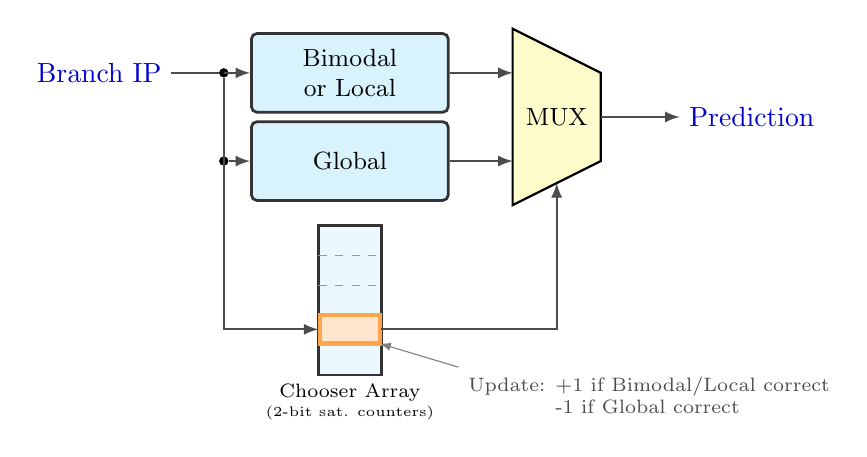
\begin{tikzpicture}[
      box/.style={draw=black!80, line width=1pt, minimum height=1cm, minimum width=2.5cm, fill=cyan!15, rounded corners=2pt, font=\small},
      arrow/.style={-latex, thick, draw=black!70},
      data_connector/.style={circle, fill=black, inner sep=1.2pt}
    ]

      % MUX using circuitikz muxdemux
      \node[muxdemux, muxdemux def={Lh=4, Rh=2, NL=2, NB=1, w=2},
            external pins width=0, fill=yellow!20, anchor=lpin 2] (mux) {};

      % Bimodal or Local box
      \node[box, align=center, left=0.8cm of mux.lpin 1, anchor=east] (bimodal) {Bimodal\\or Local};

      % Branch IP input
      \node[font=\normalsize, text=blue!80!black, left=1cm of bimodal.west] (branch_ip) {Branch IP};

      % Connector for Branch IP
      \node[data_connector, right=0.6cm of branch_ip.east] (conn) {};

      % Global box
      \node[box, left=0.8cm of mux.lpin 2] (global) {Global};

      % Chooser array - drawn with loop and dashed lines, closer to global
      \coordinate (array_start) at ([yshift=-0.3cm]global.south);

      % Draw array box outline - smaller
      \draw[draw=black!80, line width=1pt, fill=cyan!8]
        ([xshift=-0.4cm]array_start) rectangle ++(0.8cm, -1.9cm)
        node[pos=0.5] (chooser_center) {};

      % Draw dashed lines to show array elements - aligned properly
      \foreach \i in {1,2,3,4} {
        \draw[dashed, black!40] ([xshift=-0.4cm, yshift=-\i*0.38cm]array_start) -- ++(0.8cm, 0);
      }

      % Highlight one element in the middle - aligned with dashed lines
      \draw[draw=orange!70, line width=1.5pt, fill=orange!20]
        ([xshift=-0.38cm, yshift=-1.14cm]array_start) rectangle ++(0.76cm, -0.36cm)
        coordinate[pos=1] (highlight_se);

      % Label for chooser array - BELOW the array
      \node[below=0.8cm of chooser_center.south, font=\scriptsize, text=black, align=center, anchor=north]
        {Chooser Array\\[-1pt]\tiny (2-bit sat. counters)};

      % Store chooser position for connections
      \coordinate (chooser_west) at ([xshift=-0.4cm, yshift=-1.32cm]array_start);
      \coordinate (chooser_east) at ([xshift=0.4cm, yshift=-1.32cm]array_start);

      % Label for MUX
      \node at (mux.center) [font=\small] {MUX};

      % Prediction output
      \node[right=1cm of mux.rpin 1, font=\normalsize, text=blue!80!black] (prediction) {Prediction};

      % Arrows - Branch IP to all three components
      \draw[thick, draw=black!70] (branch_ip) -- (conn);
      \draw[arrow] (conn) |- (bimodal.west);
      \node[data_connector] (conn2) at (conn |- global.west) {};
      \draw[thick, draw=black!70] (conn) -- (conn2);
      \draw[arrow] (conn2) -- (global.west);
      \draw[arrow] (conn) |- (chooser_west);

      % Arrows - from predictors to MUX
      \draw[arrow] (bimodal.east) -- ++(0.3, 0) |- (mux.lpin 1);
      \draw[arrow] (global.east) -- ++(0.3, 0) |- (mux.lpin 2);

      % Arrow - Chooser to MUX control (bottom pin)
      \draw[arrow] (chooser_east) -| (mux.bpin 1);

      % Arrow - MUX to Prediction
      \draw[arrow] (mux.rpin 1) -- (prediction);

      % Add update explanation right below the highlighted box
      \node[anchor=north west, font=\scriptsize, text=black!70, align=left] (update_text)
        at ([xshift=1cm, yshift=-0.3cm]highlight_se) {
        Update: +1 if Bimodal/Local correct\\
        \phantom{Update: }-1 if Global correct
      };

      % Arrow from text to highlighted box
      \draw[-latex, draw=black!50, thin] (update_text.north west) -- (highlight_se);

    \end{tikzpicture}
  \end{center}

  \vspace{0.3em}

  \begin{itemize}\small
    \item The chooser selects which predictor to use via the MUX
    \item Each counter tracks which predictor performs better for that branch
    \item The chooser may also be indexed by the Global History Register (GHR)
  \end{itemize}
\end{frame}

% Slide 4: Example Program
\begin{frame}[fragile]
  \frametitle{Example: Nested Loop with Switch}
  
  \begin{tcolorbox}[colback=gray!5, colframe=gray!50]
    \small\ttfamily
    \begin{tabbing}
    \hspace{1em}\=\hspace{1em}\=\hspace{1em}\=\hspace{1em}\=\kill
    for (i=100; i>0; i--)\tikzmark{br0} \textcolor{blue}{$\leftarrow$ Branch 0}\\
    \> for (j=2; j<6; j++)\tikzmark{br1} \textcolor{blue}{$\leftarrow$ Branch 1}\\
    \> \> switch (i\%j) \{ \\
    \> \> \> case 0: ...\tikzmark{br2} \textcolor{blue}{$\leftarrow$ Branch 2}\\
    \> \> \> case 1: ...\tikzmark{br3} \textcolor{blue}{$\leftarrow$ Branch 3}\\
    \> \> \> case 2: ...\tikzmark{br4} \textcolor{blue}{$\leftarrow$ Branch 4}\\
    \> \> \> case 3: ...\tikzmark{br5} \textcolor{blue}{$\leftarrow$ Branch 5}\\
    \> \> \> case 4: ...\tikzmark{br6} \textcolor{blue}{$\leftarrow$ Branch 6}\\
    \> \> \}
    \end{tabbing}
  \end{tcolorbox}
    
\end{frame}

% Slide 5: Branch Behavior Patterns
\begin{frame}
  \frametitle{Branch Behavior Patterns in the Program}
  
  \scriptsize
  
  \begin{tcolorbox}[colback=gray!5, colframe=gray!50]
    \textbf{Branch 0:} TTTT...TTTN (mostly taken, rarely not taken) \\
    \vspace{0.2em}
    \textbf{Branch 1:} TTTNTTTNTTTNTTT... (periodic pattern with N)\\
    \vspace{0.2em}
    \textbf{Branch 2:} TTTTNTTTTNTTNTN... (more complex pattern)\\
    \vspace{0.2em}
    \textbf{Branch 3:} NNNNTTTTNTTTTNTT... (mixed pattern)\\
    \vspace{0.2em}
    \textbf{Branch 4:} TTTTTNNNTTTTTTTT... (clusters of N within T)\\
    \vspace{0.2em}
    \textbf{Branch 5:} TTTTTTTTTTNNTTT... (mostly T with occasional N)\\
    \vspace{0.2em}
    \textbf{Branch 6:} TTTTTTTTTTTTTTTN... (almost always taken)
  \end{tcolorbox}
  
  \normalsize
  \vspace{0.5em}
  Key observations:
  \begin{itemize}
    \item Different branches exhibit different patterns
    \item Some branches have regular patterns (0, 6)
    \item Others have complex, hard-to-predict patterns (2, 3)
    \item Pattern complexity affects prediction accuracy
  \end{itemize}
\end{frame}

% Slide 6: Performance Comparison
\begin{frame}
  \frametitle{Prediction Accuracy Comparison (5-instruction history)}
  
  \begin{columns}[T]
    \column{0.5\textwidth}
    \footnotesize
    \begin{tabular}{|l|c|}
      \hline
      \textbf{Predictor Type} & \textbf{Avg Accuracy} \\
      \hline
      \textcolor{blue}{2-bit counter} & \textcolor{blue}{76.7\%} \\
      Global history \& table & 79.9\% \\
      Local history, global table & 82.9\% \\
      Local history \& tables & 82.1\% \\
      \textcolor{red}{Global history, local tables} & \textcolor{red}{\textbf{83.5\%}} \\
      \hline
    \end{tabular}
    
    \vspace{0.5em}
    \footnotesize
    \textbf{Best performer:} Global history with local tables
    
    \column{0.5\textwidth}
    \begin{center}
      \textbf{Per-Branch Accuracy}\\[0.5em]
      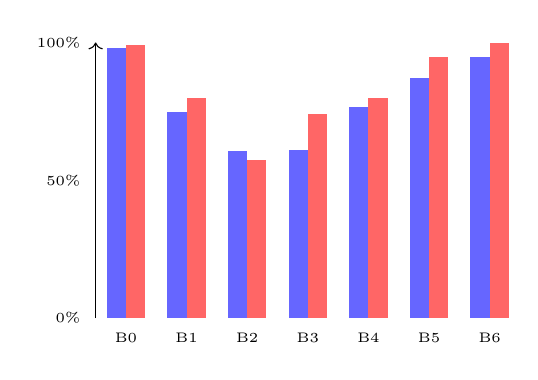
\begin{tikzpicture}[scale=0.7]
        % Draw bars for comparison
        \foreach \branch/\simple/\local in {
          0/98/99,
          1/74.75/79.75,
          2/60.5/57.25,
          3/61/74,
          4/76.75/79.75,
          5/87.25/94.75,
          6/94.75/99.75
        } {
          % Simple predictor bar
          \fill[blue!60] (\branch*1.1, 0) rectangle (\branch*1.1+0.35, \simple/20);
          % Local predictor bar
          \fill[red!60] (\branch*1.1+0.35, 0) rectangle (\branch*1.1+0.7, \local/20);
          % Branch label
          \node[below] at (\branch*1.1+0.35, -0.1) {\tiny B\branch};
        }
        % Y-axis
        \draw[->] (-0.2, 0) -- (-0.2, 5);
        \foreach \y in {0,50,100} {
          \node[left] at (-0.3, \y/20) {\tiny \y\%};
        }
      \end{tikzpicture}
    \end{center}
  \end{columns}
\end{frame}

% Slide 7: Performance Metrics
\begin{frame}
  \frametitle{Performance Metrics}
  
  \begin{center}
    \footnotesize
    \begin{tabular}{|l|c|c|c|}
      \hline
      \textbf{Configuration} & \textbf{Hit Rate} & \textbf{Cycles} & \textbf{Speedup} \\
      \hline
      All wrong & 0.0\% & 1,600,005 & baseline \\
      2-bit counter & 79.0\% & 1,126,005 & 1.42$\times$ \\
      Global history & 79.9\% & 1,120,842 & 1.43$\times$ \\
      Local hist, global table & 82.9\% & 1,102,434 & 1.45$\times$ \\
      Local hist \& tables & 82.9\% & 1,102,434 & 1.45$\times$ \\
      Global hist + local table & 83.5\% & 1,098,594 & 1.46$\times$ \\
      Perfect & 100.0\% & 1,000,005 & 1.60$\times$ \\
      \hline
    \end{tabular}
  \end{center}
  
  \vspace{1em}
  
  \begin{tcolorbox}[colback=yellow!10, colframe=yellow!50]
    \textbf{Test Parameters:}
    \begin{itemize}
      \item Instructions: 1,000,000
      \item Pipeline length: 5
      \item Misprediction penalty: 3 cycles
      \item Branch probability: 20\%
    \end{itemize}
  \end{tcolorbox}
  
  \textbf{Key Insight:} Even modest improvements in prediction accuracy (76\% → 81\%) yield significant performance gains
\end{frame}

\end{document}